\documentclass[12pt]{paper}
\usepackage{amsmath}
\usepackage{amssymb}
\usepackage{graphicx}
\usepackage{hyperref}
\usepackage{color}
\usepackage{float}
\begin{document}	
\title{A model for UV dose dependent histone sliding}
\maketitle

We set the total length of the chromatin in the initial damage region to be $l$, the number of histones in the damage region embedded in $l$ is $N(t)$, the average number of histones per unit chromatin length is thus $N(t)/l$, we set $\bar{D}$ to be the average number of damage points per unit chromatin length. We set $R(t)$ to be the expansion factor for the radius of the damage region, assuming radially symmetric expansion, $t$ the time, and $t_s$ the time at which expansion saturates. 

\textbf{Assumptions:} 
\begin{enumerate}
	\item The rate at which the number of histones change in $l$ is proportional to the number of damages per nucleosome;
	\item the rate of expansion is negatively proportional to the rate of change in the number of histones on $l$;
	\item the average number of damage points per unit chromatin length is an increasing function of the UV dose. 
\end{enumerate}

Assumption 1 can be formulated as 
\begin{equation*}
\frac{dN(t)}{dt} = -k_n\frac{\bar{D}N(t)}{l}
\end{equation*}
with $k_r$ the rate constant and the minus sign indicating depletion from damage region due to sliding. Using the initial condition $N(0) = N_0$, the solution is given by 
\begin{equation}\label{eq:NumHistones}
N(t) = N_0\exp(-\frac{k_r\bar{D}t}{l})
\end{equation}
We note that even if the linker DNA between histones is long, then sliding a histone along the linker does not change the average number of damages on the DNA wrapped around it. If sliding rate is much faster than repair rate (indeed, as evident from the experimental data), then the histone will keep on sliding until it reaches an area of the chromatin with no damages. We therefore consider the derivative of the number of histones in the damage region to be proportional to the number of damages per nucleosomes.  

From assumption 2 we can write 
\begin{equation*}
\frac{dR(t)}{dt}=-k_R\frac{dN(t)}{dt}
\end{equation*}
with the initial condition $R(0)=1$ we find 
\begin{equation}\label{eq:expansionFactor}
R(t) = 1+k_RN_0(1-\exp(-\frac{k_r\bar{D}t}{l}))
\end{equation}
with $k_R$ the rate constant.

The expansion of chromatin post UVC is attributed to two processes, one sliding from the damage region and the other is repair protein crowding. Throughout the process of expansion repair proteins keep binding to exposed damages on the DNA. Furthermore, sliding of histones causes the exposure of more damage points which are eventually bounded by repair proteins. Repair proteins' presence in the damage region produces pushing force radially outward, and cause an expansion of the damage region. The amount of repair proteins is directly proportional to the number of exposed damage points, which in turn is proportional to the number of histones in the damage region. We therefore base the justification of assumption 2 on the description provided above. 

The fraction of histone loss is given by   
\begin{equation}\label{eq:histoneLoss}
h(t) = \frac{R(t)-1}{R(t)} +\frac{N_0-N(t)}{N_0R(t)}=1-\frac{N(t)}{N_0R(t)}
\end{equation}
Substituting the expressions in \ref{eq:NumHistones} and \ref{eq:expansionFactor} into \ref{eq:histoneLoss} and setting $t=t_s$ we obtain 
\begin{equation}\label{eq:totalHistoneLoss}
h(t_s)=1-\frac{\exp(-\frac{k_r\bar{D}}{l}t_s)}{ 1+k_RN_0(1-\exp(-\frac{k_r\bar{D}}{l}t_s))}
\end{equation}

The expression on the right-hand side of \ref{eq:totalHistoneLoss} can now be regarded as function of the average number of damage points per unit length, $\bar{D}$. Using assumption 3 above, $\bar{D}$ increases with the UV dose at least linearly and decreases with the distance from focal point, as evident from experimental data. The decrease of UVC intensity, $I$, with distance from the its focal point is assumed to follow the inverse-square law of laser intensity. That is, $I\propto U/r^2$, with $r$ the distance from focal point, and $U$ the uv exposure time. 

Assuming a uniform distribution of DNA, the amount of DNA enclosed in concentric rings around the focal point increases linearly with $r$. Therefore, the expected number of damages in each concentric ring is $D\propto rU/r^2=U/r$. 
The average of $\bar{D}$ in a circular region of radius $R$ is then proportional to 
\begin{equation}
\bar{D}(R)\propto \int_0^R Ur/r dr = UR
\end{equation}
and the average number of damages per unit length is thus proportional to $U$.

We therefore substitute this estimation into \ref{eq:totalHistoneLoss} to obtain the total loss of histones as a function of the UV dose at $t_{s}$
\begin{equation}\label{eq:totalHiostoneLossVsUV}
h(t_s;U)=1-\frac{\exp(-\frac{k_rt_s}{l}U)}{ 1+k_RN_0(1-\exp(-\frac{k_rt_s}{l}U))}
\end{equation}
 
The DNA loss at $t_{s}$ is a function of the expansion factor $R(t)$ and is given by 
\begin{equation}\label{eq:dStSt}
d(t_s)= 1-1/R(t_s) 
\end{equation}
substituting the expression from \ref{eq:expansionFactor} into \ref{eq:dStSt}, we obtain 
\begin{equation}\label{eq:dnaLoss}
d(t_s;U) =  \frac{k_RN_0(1-\exp(-\frac{k_rt_s}{l}U))}{(1+k_RN_0(1-\exp(-\frac{k_rt_s}{l}U)))}
\end{equation}
which is also regarded as a function of the UV dose. 

Both $h(t_s;U)$ and $d(t_s;U)$ share similar parameters, we therefore fit the experimental histone loss data to \ref{eq:totalHiostoneLossVsUV}, and plug the estimated parameters into the analytical expression for $d(t_s;U) $
\begin{figure}[H]
\centering
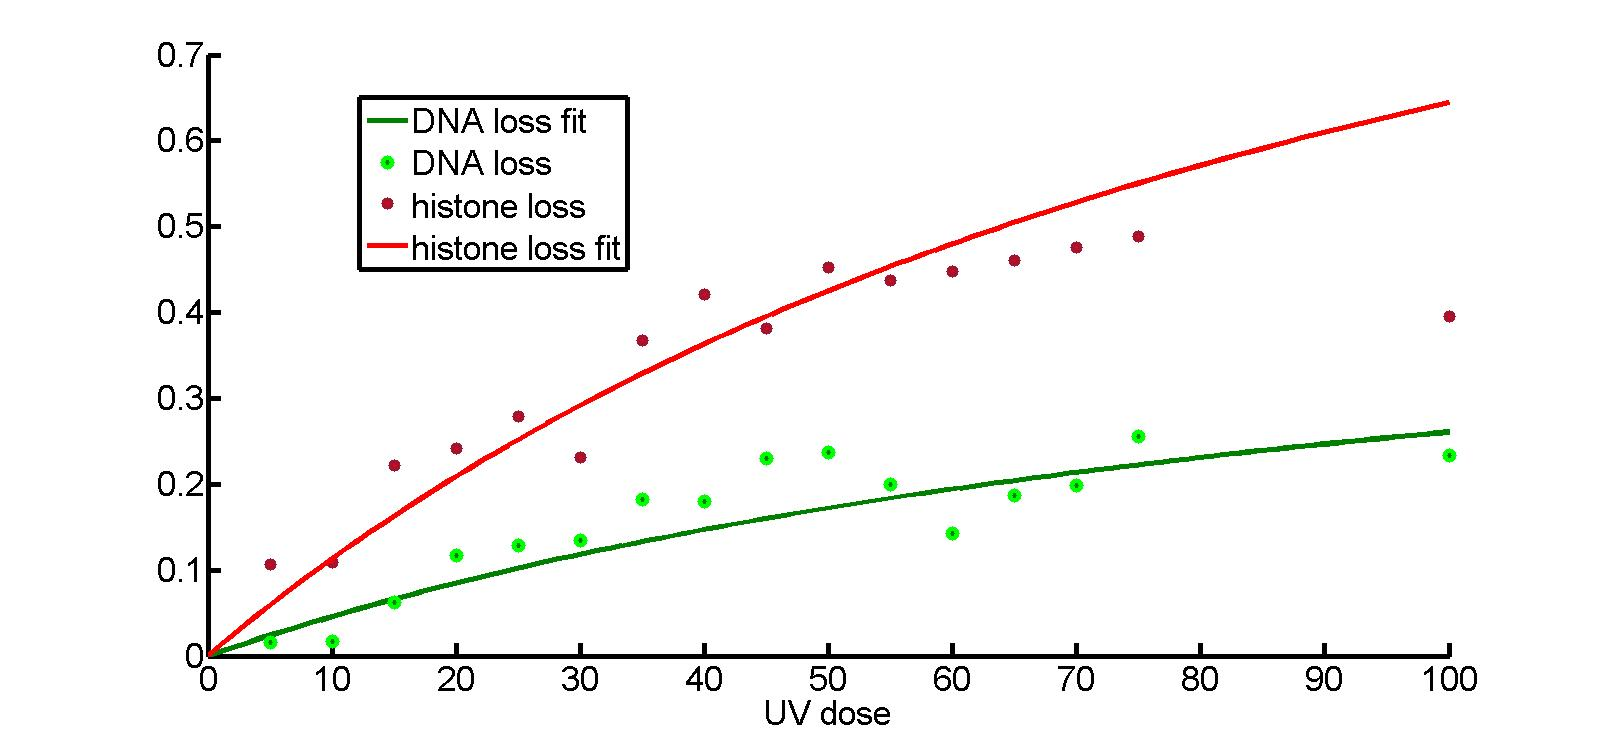
\includegraphics[width=0.5\linewidth, height=0.3\textheight]{images/histoneAndDnaVsUvDoseModelFit}
\caption{\textbf{\tiny{}Fit of the model for histone loss (red curve) to the experimental data (red circle) parameters values obtained were $K_RN_0 =0.68\quad k_rt_s/l=0.0073$. These parameter values were then plugged into equation \ref{eq:dnaLoss} and plotted (green curve) against the experimental DNA loss data (green circles)}}
\label{fig:histoneAndDnaVsUvDoseModelFit}
\end{figure}

Parameters found by this fitting are 
\begin{equation}
k_rt_s/l = 0.0073 \quad k_RN_0 = 0.68
\end{equation}
Using these parameters we find that the fraction of histones sliding out of the damage region, namely $(h-d)/(1-d)$, behaves in a near linear fashion. As evident 
in Figure \ref{fig:histoneSlideFromDamageRegionComparision}, the qualitative difference between the model and the linear fit is small, in the sense that  both capture well the increase in sliding fraction in the UV dose range of the experimental data with near equal variations from experimental data. 

\begin{figure}
\centering
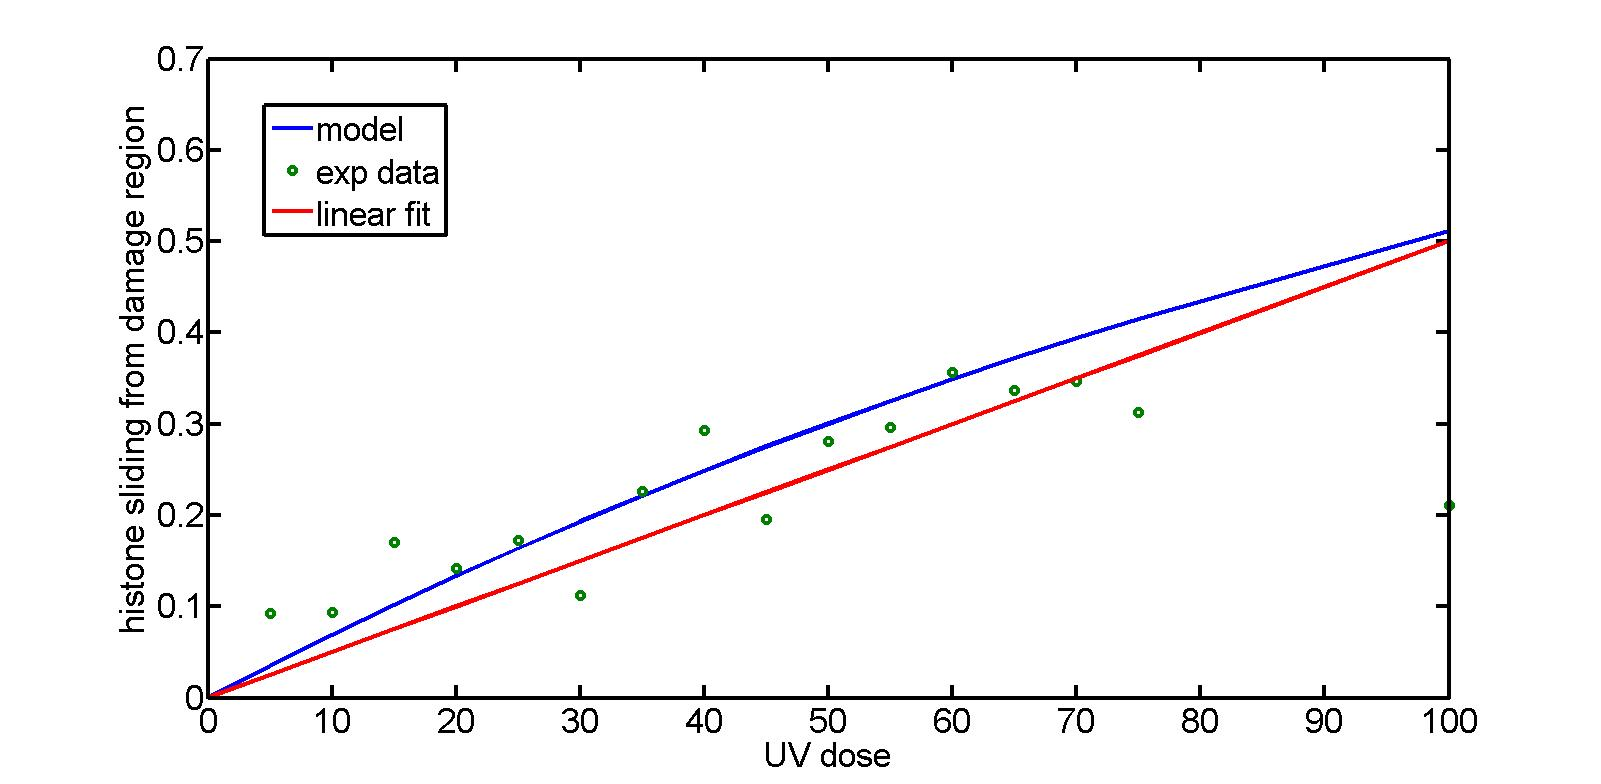
\includegraphics[width=0.7\linewidth, height=0.3\textheight]{images/histoneSlideFromDamageRegionComparision}
\caption{}
\label{fig:histoneSlideFromDamageRegionComparision}
\end{figure}



\end{document}

